\newpage

\section{Detekcja źrenic}

Do wykrywania źrenic, najpierw musimy wyznaczyć obszar oczu (patrz rozdz. \hyperref[{section:eye_detection}]{\textit{\ref{section:eye_detection}.Detekcja oczu}}. Następnie korzystając z jednych z poniższych metod ustalamy interesujący nas środek źrenicy. \\
Wynik, który w przybliżeniu chcę uzyskać:
----- jeśli będzie więcej metod to przesunąć to do testów ------

\begin{figure}[!h]
    \begin{center}
        
\includegraphics[scale=0.35]{img/pupil_section/expected_pupils.jpg}
        \caption{W przybliżeniu środek źrenic, który chcę uzyskać}
        \label{fig:expected_pupils}
    \end{center}
\end{figure}

\subsection{Algorytm CDF}
Algorytm zaimplementowany na podstawie dwóch artykułów o detekcji źrenic \cite{IMECSPupilCDFAnalysis}
\cite{EyePupilWebCam}. Opiera się w głównej mierze na progowaniu za pomocą dystrybuanty. Cały algorytm przetwarza obszar oka w skali szarości. \\
Metoda ta daje całkiem dobre i prawdopodobnie wystarczające rezultaty. \\

\begin{figure}[!h]
    \begin{center}
        \subfigure[Oko skierowane w prawo]{\label{fig:pupil_cdf_left}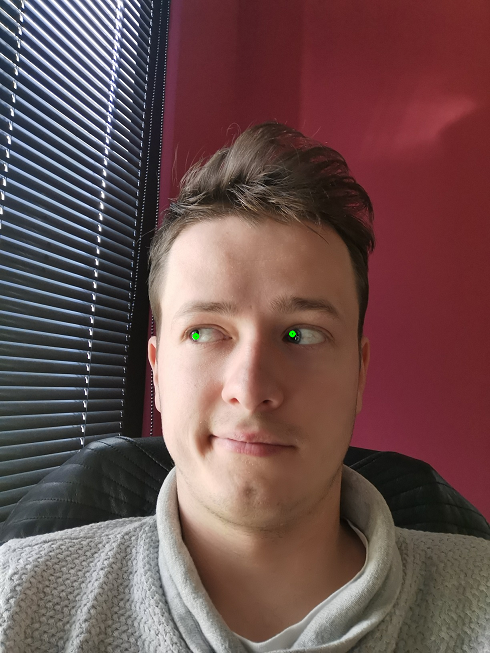
\includegraphics[scale=0.3]{img/pupil_section/pupil_2eyes_left_1.png}}
        \hspace{3mm}
        \subfigure[Oko skierowane na wprost]{\label{fig:pupil_cdf_center}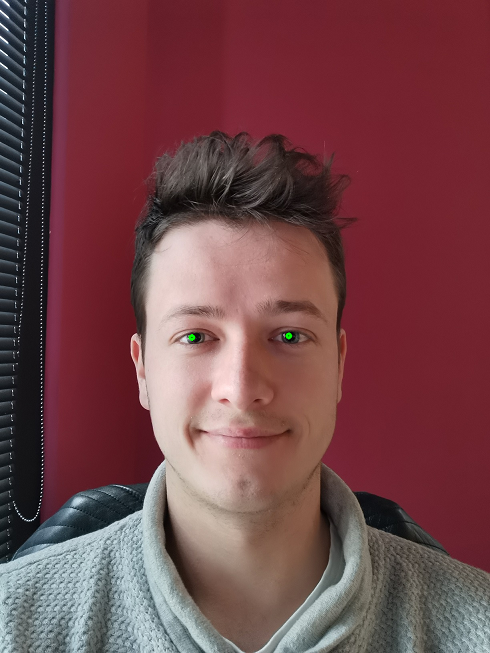
\includegraphics[scale=0.3]{img/pupil_section/pupil_2eyes_center_1.png}}
        \hspace{3mm}
        \subfigure[Oko skierowane w lewo]{\label{fig:pupil_cdf_right}
\includegraphics[scale=0.3]{img/pupil_section/pupil_2eyes_right_1.png}}
    \end{center}
    \caption{Rezultat wykrywania źrenic metodą CDF}
    \label{fig:cdf_results}
\end{figure}

\subsubsection{Kroki algorytmu}

\begin{itemize}
    \item Za pomocą progowania z użyciem dystrybuanty tworzymy obraz binarny.\\
    \begin{align}
        CDF(r) = \sum_{w=0}^{r} p(w)
    \end{align}
    
    Gdzie \textit{p(w)} to prawdopodobieństwo znalezienia punktu o jasności równej \textit{w} - określone przy pomocy dystrybuanty dystrybuanty.
    
    \begin{align}
        I`(x, y) = 
        \begin{cases}
            255, &  CDF(I(x, y)) < \textit{a}\\
            0,   &  wpp
        \end{cases}
    \end{align} 
    
    Gdzie \textit{I} to jasność piksela, natomiast \textit{a} to ustalony próg

    \item Na uzyskany obraz binarny nakładamy operację morfologiczną erozji (filtr minimalny), celem usunięcia pojedynczych ciemnych pikseli
    
    \item Znajdujemy najciemniejszy piksel na oryginalnym obrazie wśród tych, które mają wartość 255 (są białe) na obrazie binarnym
    
    \item Obliczamy średnią jasność pikseli w kwadracie 10x10 wokół wybranego najciemniejszego punktu
    
    \item Nakładamy erozję na obszarze 15x15 wokół wybranego punktu
    \item Na tym obszarze stosujemy progowanie
    
    \begin{align}
        I`(x, y) = 
        \begin{cases}
            255, &  I(x, y) < AVG_I\\
            0,   &  wp.p.
        \end{cases}
    \end{align}
    
    Gdzie \textit{AVG$_I$} to średnia jasność obszaru obliczona wcześniej
    
    \item Środkiem źrenicy będzie środek ciężkości białych punktów na binarnym obszarze, który uzyskaliśmy

\end{itemize}


\begin{figure}[!h]
    \begin{center}
        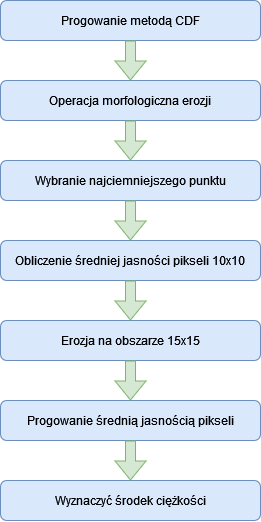
\includegraphics[scale=0.35]{img/pupil_section/CDF_Diagram.png}
        \caption{Kroki algorytmu metodą CDF}
        \label{fig:cdf_diagram}
    \end{center}
\end{figure}

\subsubsection{Wynik kolejnych etapów algorytmu}
Na \hyperref[{fig:cdf_steps}]{\textit{rysunku \ref{fig:cdf_steps}}} przedstawiony jest na przykładzie wynik kolejnych etapów detekcji źrenic za pomocą metody CDF.

\begin{figure}[!h]
    \begin{center}
        \subfigure[Obszar oka w RGB]{\label{fig:cdf_rgb}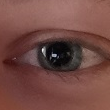
\includegraphics[scale=0.50]{img/pupil_section/CDF_steps/CDF_rgb_eye.png}}
        \hspace{8mm}
        \subfigure[Obszar oka w skali szarości]{\label{fig:cdf_gray}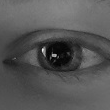
\includegraphics[scale=0.50]{img/pupil_section/CDF_steps/CDF_gray_eye.png}}
        \hspace{8mm}
        \subfigure[Wynik progowania CDF]{\label{fig:cdf_binary}
\includegraphics[scale=0.50]{img/pupil_section/CDF_steps/CDF_binary_eye_after_CDF.png}}
        
        \hfill
        
        \subfigure[Wynik erozji]{\label{fig:cdf_erode}
\includegraphics[scale=0.50]{img/pupil_section/CDF_steps/CDF_binary_eye_after_erode.png}}
        \hspace{8mm}
        \subfigure[Najciemniejszy punkt]{\label{fig:cdf_darkest}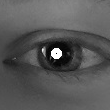
\includegraphics[scale=0.50]{img/pupil_section/CDF_steps/CDF_darkest_pixel.png}}
        \hspace{8mm}
        \subfigure[Obszar 15x15 wokół najciemniejszego punktu ]{\label{fig:cdf_pmi}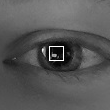
\includegraphics[scale=0.50]{img/pupil_section/CDF_steps/CDF_pmi.png}}
        
        \hfill
        
        \subfigure[Wynik erozji]{\label{fig:cdf_eroded_pmi}
\includegraphics[scale=0.50]{img/pupil_section/CDF_steps/CDF_eroded_pmi.png}}
        \hspace{8mm}
        \subfigure[Progowanie średnią jasnością pikseli]{\label{fig:cdf_threshold}
\includegraphics[scale=0.50]{img/pupil_section/CDF_steps/CDF_threshold_pmi.png}}
        \hspace{8mm}
        \subfigure[Wykryte położenie źrenicy]{\label{fig:cdf_pupil_detected}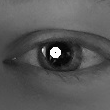
\includegraphics[scale=0.50]{img/pupil_section/CDF_steps/CDF_pupil_detected.png}}
        
    \end{center}
    \caption{Kolejne etapy wykrywania źrenic metodą CDF}
    \label{fig:cdf_steps}
\end{figure}

\subsection{Algorytm PF}
{\_\_\_\_} W przyszłości do testów zaimplementować algorytm PF\cite{EyePupilWebCam} {\_\_\_\_}

\subsection{Algorytm EA}
{\_\_\_\_} W przyszłości do testów zaimplementować algorytm EA\cite{EyePupilWebCam} {\_\_\_\_}
